<<<<<<< Updated upstream
=======
\chapter{Implementacija i korisničko sučelje}

\section{Korištene tehnologije i alati}

\paragraph{}
{Komunikacija u timu realizirana je korištenjem aplikacije WhatsApp \footnote{\url{https://https://www.whatsapp.com/}}. Za izradu UML dijagrama korišten je alat Astah Professional\footnote{\url{https://astah.net/products/astah-professional/}}, a kao sustav za upravljanje izvornim kodom Git\footnote{\url{https://git-scm.com/}}. Udaljeni repozitorij projekta dostupan je na web platformi GitHub\footnote{\url{https://github.com/}}.
}
\paragraph{}{
Kao razvojno okruženje korišten je Microsoft Visual Studio \footnote{\url{https://visualstudio.microsoft.com/}}- integrirano je razvojno sučelje (IDE) tvrtke Microsoft. Prvenstveno se koristi za razvoj računalnih programa za operacijski sustav Windows, kao i za web-stranice, web-aplikacije, web-usluge i mobilne aplikacije. Visual Studio za razvoj softvera koristi Microsoftove platforme kao što su windows API, Windows Forms, Windows Presentation Foundation, Windows Store i Microsoft Silverlight.
}
\paragraph{}{
Aplikacija je napisana koristeći radni okvir jezik C\# \footnote{\url{https://learn.microsoft.com/en-us/dotnet/csharp/tour-of-csharp/}} za izradu backenda te React \footnote{\url{https://react.dev/}} i jezik JavaScript za izradu frontenda. React, također poznat kao React.js je biblioteka u JavaScriptu za izgradnju korisničkih sučelja. Održana je od strane Facebooka. React se najčešće koristi kao osnova u razvoju web ili mobilnih aplikacija. Složene aplikacije u Reactu obično zahtijevaju korištenje dodatnih biblioteka za interakciju s API-jem. Radni okvir Baza podataka se nalazi na poslužitelju u oblaku Microsoft Azure \footnote{\url{https://azure.microsoft.com/en-us}}.
}	



\section{Ispitivanje programskog rješenja}

\section{Dijagram razmještaja}

\paragraph{}{
UML-dijagrami razmještaja (engl. deployment diagrams) prikazuju fizičku arhitekturu programskog sustava, prikazujući razmještaj programskih artefakata na sklopovskim čvorovima ili na virtualnim okruženjima.
}

\paragraph{}{
Naš se sustav bazira na ”klijent – posluzitelj” arhitekturi, te se komunikacija između računala korisnika i poslužitelja odvija pomoću HTTP veze. Pristup web aplikaciji odvija se preko web preglednika računala korisnika. Na poslužitelju se nalaze web poslužitelj i poslužitelj baze podataka.
}

\begin{figure}[!htb]
	\centering
	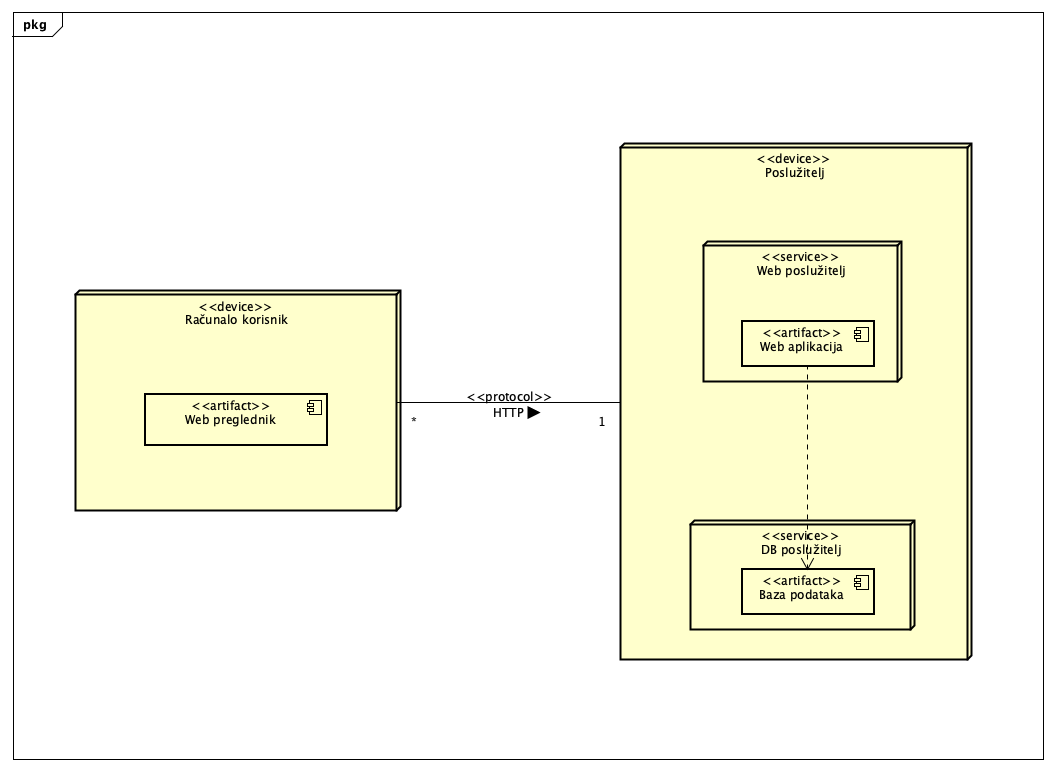
\includegraphics[width=1\linewidth]{dijagrami/DijagramRazmjestaja.png}
	\caption{Dijagram razmještaja}
	\label{fig:modelsdiagram}
\end{figure}

\section{Upute za puštanje u pogon}

\subsection{Instalacija poslužitelja baze podataka}

\paragraph{}{
	Koraci za Deployanje Aplikacije s Azure MySQL Bazom Podataka
	1. Kreiranje Azure MySQL Baze Podataka:
	Prijavite se na Azure portal koristeći odgovarajuće vjerodajnice.
	Kreirajte novu uslugu baze podataka putem Azure portal sučelja, odabravši "Create a resource" i pretražujući "Azure Database for MySQL".
	Unesite potrebne informacije za konfiguraciju baze podataka, uključujući ime, korisničko ime, lozinku i druge relevantne parametre.
	Kreirajte bazu podataka i sačuvajte informacije o povezivanju (hostname, port, korisničko ime, lozinka) za buduće konfiguracije.
	2. Povezivanje s Azure MySQL Bazom Podataka iz MySQL Workbencha:
	Otvorite MySQL Workbench na lokalnom računalu.
	Konfigurirajte novu vezu prema Azure MySQL bazi podataka koristeći informacije o povezivanju dobivene u prethodnom koraku.
	Testirajte vezu kako biste potvrdili ispravnost postavki.
	3. Konfiguracija Aplikacije za Azure MySQL Bazu Podataka:
	U izvornom kodu aplikacije (npr. persistence.xml datoteka), promijenite postavke vezane uz bazu podataka kako bi odražavale parametre Azure MySQL baze podataka.
	Prilagodite korisničko ime, lozinku, hostname i port prema informacijama dobivenim prilikom konfiguracije Azure MySQL baze podataka.
	4. Pakiranje Aplikacije:
	Koristite alate poput Mavena ili Gradlea kako biste pakirali web aplikaciju u WAR (Web Application Archive) datoteku.
	5. Deploy na Azure:
	Prijavite se na Azure portal.
	Kreirajte novi "Web App" koji će hostati vašu aplikaciju.
	U postavkama web app-a, odaberite opciju "Deployment Center" i povežite se s odabranim repozitorijem (npr. Git, Azure Repos).
	Konfigurirajte deployment postavke kako bi Azure automatski pokrenuo skripte za konfiguraciju i deploy aplikacije.
	6. Konfiguracija Veze s Bazom Podataka na Azure-u:
	U postavkama web app-a na Azure portalu, pronađite odjeljak za konfiguraciju i postavite varijable okoline koje su potrebne za povezivanje s Azure MySQL bazom podataka (npr. MYSQLCONNSTR varijable).
	7. Pokretanje Aplikacije:
	Provjerite status deploya na Azure portalu.
	Aplikaciju možete pokrenuti pristupanjem pristupnoj adresi koja je dostupna putem Azure web app-a.
}




\eject
>>>>>>> Stashed changes
